%%%%%%%%%%%%%%%%%%%%%%%%%%%%%%%%%%%%%%%%%%%%%%%%%%%%%%%%%%%%%%%%%%%%%%%%%%%%%%%%%%
\begin{frame}[fragile]\frametitle{}
\begin{center}
{\Large Samadhi Paad समाधिपाद}
\end{center}
\end{frame}


%%%%%%%%%%%%%%%%%%%%%%%%%%%%%%%%%%%%%%%%%%%%%%%%%%%%%%%%%%%
\begin{frame}[fragile]\frametitle{Introduction}


	\begin{itemize}
	\item Samadhi refers to a blissful state of existence that is believed to be even beyond mind and meditation.
	\item In this chapter, the author describes yoga and then our true nature and then he instructs the means to attain Samadhi. 
	\item Patanjali begins this chapter with a definition of yoga.
	\item He lists the obstacles we may encounter to attaining mental silence. 
	\item But, having overcome such obstacles, he explains what it is like when we have achieved mental silence as well.
	\end{itemize}

\tiny{(Ref: Basic Introduction of Patanjali Yoga Sutras – The Best Knowledge for Yogis - Yoga Moha)}

\end{frame}

%%%%%%%%%%%%%%%%%%%%%%%%%%%%%%%%%%%%%%%%%%%%%%%%%%%%%%%%%%%
\begin{frame}[fragile]\frametitle{Types of Samadhi समाधी}

\begin{center}
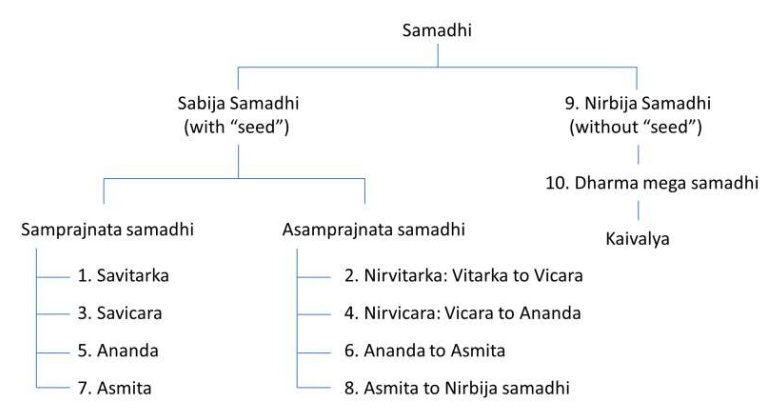
\includegraphics[width=\linewidth,keepaspectratio]{yog37}

\end{center}

  
  \tiny{(Ref: Patanjali Yoga Darshan- For AYUSH YOGA EXAM- Deepak D.Khaire)}

\end{frame}


%%%%%%%%%%%%%%%%%%%%%%%%%%%%%%%%%%%%%%%%%%%%%%%%%%%%%%%%%%%
\begin{frame}[fragile]\frametitle{The Beginning}

\begin{sanskrit}
अथ योग अनुशासनम् ॥१॥
\end{sanskrit}


	\begin{itemize}
	\item अथ primarily means `now' has many levels of meanings.
		\begin{itemize}
		\item You have done lots of reading, getting knowledge, NOW, lets practice Yog
		\item You have been coming from different evolutionary paths, NOW you are eligible to do Yog
		\item अनुशासनम् means discipline. अनु means following. Now follow the Yog tradition. Meaning Yog was known before (like in Gita), NOW its time to continue/follow it.
		\end{itemize}	
	\item [HA]: Now Then Yoga Is Being Explained.
	\item [IT]: Now, an exposition of Yoga (is to be made).
	\item [VH]: Now, the instructions of Yoga.
	\item [BM]: This is the teaching of yoga.
	\item [SS]: Now the exposition of Yoga is being made.
	\item [SP]: This is the beginning of instruction in yoga.
	\item [SV]: Now concentration is explained
	\end{itemize}

\end{frame}


%%%%%%%%%%%%%%%%%%%%%%%%%%%%%%%%%%%%%%%%%%%%%%%%%%%%%%%%%%%
\begin{frame}[fragile]\frametitle{Definition of Yog}

\begin{sanskrit}
योग: चित्तवृत्ति निरोध:  ॥२॥
\end{sanskrit}

	\begin{itemize}
	\item Yog is complete cessation/stilling of perturbations of mind
	\item चित (chit): to enlighten to know, to make aware (जाणणे/जानना)
	\item चित्त (chitta): the enlightened, all inclusive term, different faculties of mind.
	\item Reality: This is much easier said than done. 
	\item During meditation a cloud of thoughts rolls in like a storm or a swarm of mosquitoes. This can be addressed by acts of observations. \item Awareness itself is our true nature and that the temporary buzz of thoughts, feelings, and sensations is not real or significant. ({\tiny Ref: Rodney Yee Decodes Yoga Sutra 1.2: Calm the Chatter of the Mind})
	\end{itemize}

\end{frame}


%%%%%%%%%%%%%%%%%%%%%%%%%%%%%%%%%%%%%%%%%%%%%%%%%%%%%%%%%%%
\begin{frame}[fragile]\frametitle{चित्त}

\begin{sanskrit}
योग: चित्तवृत्ति निरोध:  ॥२॥
\end{sanskrit}

	\begin{itemize}
	\item अन्त:करण : मन, बुद्धि, अहंकार, चित्त
	\item Chitta is like a river, flowing in two opposite directions: worldliness to/from Kaivalya कैवल्य (व्यास भाष्य)
	\item Levels of Chitta:
		\begin{itemize}
		\item मूढ चित्त  Dull, intertial, Tamas तमस
		\item क्षिप्त चित्त  Restless, distracted, Rajas  रजस
		\item विक्षिप्त चित्त Sometimes steady Sattva सत्व
		\item एकाग्र चित्त Focused
		\item निरुद्ध चित्त Restricted
		\end{itemize}
	\item [HA]: Yoga Is The Suppression Of The Modifications Of The Mind
	\item [IT]: Yoga is the inhibition of the modifications of the mind.
	\item [VH]: Yoga is the nirodha (process of ending) of the vrrti (definitions) of citta (field of consciousness.
	\item [BM]: Yoga is the cessation of the turnings of thought.
	\item [SS]: The restraint of the modifications of the mind-stuff is Yoga.
	\item [SP]: Yoga is the control of thought-waves in the mind.
	\item [SV]: Yoga is restraining the mind – stuff (Chitta) from taking various forms (Vrittis).
	\end{itemize}

\end{frame}

%%%%%%%%%%%%%%%%%%%%%%%%%%%%%%%%%%%%%%%%%%%%%%%%%%%%%%%%%%%
\begin{frame}[fragile]\frametitle{Essence of Yog}

\begin{sanskrit}
तदा द्रष्टु: स्वरुपे अवस्थानम् ॥३॥
\end{sanskrit}


	\begin{itemize}
	\item Yog is complete cessation/stilling of perturbations of mind
	\item [HA]: Then The Seer Abides In Itself
	\item [IT]: Then the Seer is established in his own essential nature.
	\item [VH]: Then, the abidance of (I) the seer (drastr) in (my) own nature (svarupa)
	\item [BM]: When thought ceases, the spirit stands in it’s true identity as observer to the world.
	\item [SS]: Then the Seer [Self] abides in His own nature.
	\item [SP]: Then man abides in his real nature.
	\item [SV]: At that time (the time of concentration) the seer (Purusha) rests in his own (unmodified) state.	
	\end{itemize}

\end{frame}

%%%%%%%%%%%%%%%%%%%%%%%%%%%%%%%%%%%%%%%%%%%%%%%%%%%%%%%%%%%
\begin{frame}[fragile]\frametitle{Essence of Yog}

\begin{sanskrit}
वृत्ति सारुप्यं इतरत्र ॥४॥
\end{sanskrit}


	\begin{itemize}
	\item Once the stilling happens, Then the seer (Purush, पुरुष ) gets to see his own true nature.
	\item Till that time, there is a continual identification with vruttis वृत्ति like reflection of the moon in the lake.
	\item Essence of Yog: still the mind-lake, to see the true bottom.
	\item [HA]: At Other Times The Seer Appears To Assume The Form Of The Modifications Of The Mind
	\item [IT]: In other states there is assimilation (of the Seer) with the modifications (of the mind)
	\item [VH]: Otherwise there is conformity to the vrrti-definitions.
	\item [BM]: Otherwise, the observer identifies with the turnings of thought.
	\item [SS]: At other times [the Self appears to] assume the forms of mental modifications.
	\item [SP]: At other times, when he is not in the state of yoga, man remains identified with the thought-waves in the mind.
	\item [SV]: At other times (other than that of concentration) the seer is identified with the modifications.	
	\end{itemize}

\end{frame}


%%%%%%%%%%%%%%%%%%%%%%%%%%%%%%%%%%%%%%%%%%%%%%%%%%%%%%%%%%%
\begin{frame}[fragile]\frametitle{वृत्ति}

\begin{sanskrit}
वृत्तय: पञ्चतय्य: क्लिष्टा अक्लिष्टा ॥५॥
\end{sanskrit}


	\begin{itemize}
	\item 5 types of vruttis : painful/complicated and not complicated
	\item प्रमाणं विपर्यय विकल्प निद्रा स्मृतय: १.०६
		\begin{itemize}
		\item प्रमाणं : यथार्थ ज्ञान : correct knowledge with right perception
		\item विपर्यय : भ्रामक ज्ञान : False knowledge
		\item विकल्प : काल्पनिक ज्ञान : Imaginary knowledge
		\item निद्रा : अभाव ज्ञान : Lack of knowledge
		\item स्मृति : Memory
		\end{itemize}	
	\item [HA]: They Fall Into Five Varieties Of Which Some Are ‘Klista’ And The Rest are ‘Aklista’.
	\item [IT]: The modifications of the mind are five-fold and are painful and not-painful.
	\item [VH]: Vrrti-definitions are five-fold. They are either klista-obstructing (causing pain) or aklista-non-obstructing (not causing pain)
	\item [BM]: The turnings of thought, whether corrupted or immune to the forces of corruption, are of five kinds.
	\item [SS]: There are five kinds of mental modifications which are either painful or painless.
	\item [SP]: There are five kinds of thought-waves—some painful, others not painful.
	\item [SV]: There are five classes of modifications, (some) painful and (others) not painful.
	\end{itemize}

\end{frame}


%%%%%%%%%%%%%%%%%%%%%%%%%%%%%%%%%%%%%%%%%%%%%%%%%%%%%%%%%%%
\begin{frame}[fragile]\frametitle{वृत्ति}

\begin{sanskrit}
 प्रमाणं विपर्यय विकल्प निद्रा स्मृतय: ॥६॥
\end{sanskrit}


\begin{itemize}
\item प्रमाणं : यथार्थ ज्ञान : correct knowledge with right perception
\item विपर्यय : भ्रामक ज्ञान : False knowledge
\item विकल्प : काल्पनिक ज्ञान : Imaginary knowledge
\item निद्रा : अभाव ज्ञान : Lack of knowledge
\item स्मृति : Memory
\item [HA]: Pramana, Viparyaya, Vikalpa, Sleep and Recollection
\item [IT]: (They are) right knowledge, wrong knowledge, fancy, sleep and memory.
\item [VH]: They are: evaluation, misperception, conceptualization, sleep and memory.
\item [BM]: They are valid judgment, error, conceptualization, sleep and memory.
\item [SS]: They are right knowledge, misconception, verbal delusion, sleep and memory.
\item [SP]: These five kinds of thought-waves are: right knowledge, wrong knowledge, verbal delusion, sleep and memory.
\item [SV]: (These are) right knowledge, indiscrimination, verbal delusion, sleep, and memory.
\end{itemize}	

\end{frame}



%%%%%%%%%%%%%%%%%%%%%%%%%%%%%%%%%%%%%%%%%%%%%%%%%%%%%%%%%%%
\begin{frame}[fragile]\frametitle{चित्त वृत्ति}

\begin{sanskrit}
प्रत्यक्ष अनुमान आगम: प्रमाणानि ॥७॥
\end{sanskrit}


	\begin{itemize}
	\item Correct knowledge is obtained through direct perception
	\item Incorrect knowledge is based on false perception, eg rope looks like a snake in the dark
	\item Verbal knowledge which does not have actual object is imaginary knowledge eg horn of rabbit
	\item [HA]: Perception, Inference And Testimony Constitute the Pramanas.
	\item [IT]: (Facts of ) right knowledge (are based on) direct cognition, inference or testimony.
	\item [VH]: Pramana-valid means of evaluation are: Direct perception, inference, and testimony.
	\item [BM]: The valid means of judgment are direct perception, inference, and verbal testimony.
	\item [SS]: The sources of right knowledge are direct perception, inference and scriptural testimony.
	\item [SP]: The right kinds of knowledge are: direct perception, inference and scriptural testimony.
	\item [SV]: Direct perception, inference, and competent evidence are proofs.
	\end{itemize}

\end{frame}


%%%%%%%%%%%%%%%%%%%%%%%%%%%%%%%%%%%%%%%%%%%%%%%%%%%%%%%%%%%
\begin{frame}[fragile]\frametitle{चित्त वृत्ति}

\begin{sanskrit}
विपर्यय: मिथ्या ज्ञानम् अतद् रूप प्रतिष्ठम् ॥८॥
\end{sanskrit}


	\begin{itemize}
	\item Correct knowledge is obtained through direct perception
	\item Incorrect knowledge is based on false perception, eg rope looks like a snake in the dark
	\item Verbal knowledge which does not have actual object is imaginary knowledge eg horn of rabbit
	\item [HA]: Viparyaya Or Illusion Is False Knowledge Formed Of A Thing As Other Than What It Is.
	\item [IT]: Wrong knowledge is a false conception of a thing whose real form does not correspond to such a mistaken conception.
	\item [VH]: Viparyaya-misperception is mistaken knowledge, founded on an appearance which is not that.
	\item [BM]: Error is false knowledge with no objective basis.
	\item [SS]: Misconception occurs when knowledge of something is not based upon its true form.
	\item [SP]: Wrong knowledge is knowledge which is false and not based upon the true nature of its object.
	\item [SV]: Indiscrimination is false knowledge not established in real nature.
	\end{itemize}

\end{frame}

%%%%%%%%%%%%%%%%%%%%%%%%%%%%%%%%%%%%%%%%%%%%%%%%%%%%%%%%%%%
\begin{frame}[fragile]\frametitle{चित्त वृत्ति}

\begin{sanskrit}
शब्द ज्ञान अनुपाति वस्तु शून्यो विकल्प: ॥९॥
\end{sanskrit}


	\begin{itemize}
	\item Correct knowledge is obtained through direct perception
	\item Incorrect knowledge is based on false perception, eg rope looks like a snake in the dark
	\item Verbal knowledge which does not have actual object is imaginary knowledge eg horn of rabbit
	\item [HA]: The Modification Called ‘Vikalpa’ Is Bases On Verbal Cognition In Regard To A Thing Which Does Not Exists. (It is a Kind Of Useful Knowledge Arising Out Of A Meaning Of A Work But Having No Corresponding Reality)
	\item [IT]: An image conjured up by words without any substance behind it is fancy.
	\item [VH]: Vikalpa-conceptualization is without an (actual) object – relying upon concept in language.
	\item [BM]: Conceptualization comes from words devoid of substance.
	\item [SS]: An image that arises on hearing mere words without any reality [as it’s base] is verbal delusion.
	\item [SP]: Verbal delusion arises when words do not correspond to reality.
	\item [SV]: Verbal delusion follows from words having no (corresponding) reality.
	\end{itemize}

\end{frame}

%%%%%%%%%%%%%%%%%%%%%%%%%%%%%%%%%%%%%%%%%%%%%%%%%%%%%%%%%%%
\begin{frame}[fragile]\frametitle{Sleep}
\begin{sanskrit}
अभावप्रत्ययालम्बना वृत्तिर्निद्रा॥१०॥
\end{sanskrit}
	\begin{itemize}
	\item [HA]: Dreamless Sleep Is The Mental Modification Produced By Condition Of Inertia As the State Of Vacuity or Negation (Of Waking And Dreaming)
	\item [IT]: That modification of the mind which is based on the absence of any content in it is sleep.
	\item [VH]: Nidra-sleep is a vrrti depending on a pratyaya- the immediate arising thought toward non-wakefulness.
	\item [BM]: Sleep is the turning of thought abstracted from existence.
	\item [SS]: That mental modification supported by cognition of nothingness is sleep.
	\item [SP]: Sleep is a wave of thought about nothingness.
	\item [SV]: Sleep is a Vritti which embraces the feeling of voidness. 
	\end{itemize}
\end{frame}


%%%%%%%%%%%%%%%%%%%%%%%%%%%%%%%%%%%%%%%%%%%%%%%%%%%%%%%%%%%
\begin{frame}[fragile]\frametitle{Memory}
\begin{sanskrit}
अनुभूतविषयासंप्रमोषः स्मृतिः॥११॥
\end{sanskrit}

	\begin{itemize}
	\item [HA]: Recollection Is Mental Modification Caused By Reproduction Of The Previous Impression Of An Object Without Adding anything From Other Sources
	\item [IT]: Memory is not allowing an object which has been experienced to escape.
	\item [VH]: Smrti- (the act of) memory is the non-escaping of the visaya-experienced objects.
	\item [BM]: Memory is the recollection of objects one has experienced.
	\item [SS]: When a mental modification of an object previously experienced and not forgotten, comes back to consciousness, that is memory.
	\item [SP]: Memory is when perceived objects are not forgotten, but come back to consciousness.
	\item [SV]: Memory is when the (Vrittis of) perceived subjects do not slip away (and through impressions come back to consciousness. 
	\end{itemize}
\end{frame}


%%%%%%%%%%%%%%%%%%%%%%%%%%%%%%%%%%%%%%%%%%%%%%%%%%%%%%%%%%%
\begin{frame}[fragile]\frametitle{Detachment}
\begin{sanskrit}
अभ्यासवैराग्याभ्यां तन्निरोधः॥१२॥
\end{sanskrit}

	\begin{itemize}
	\item [HA]: By Practice And Detachment These Can Be Stopped.
	\item [IT]: Their suppression (is brought about) by persisitent practice and non-attachment.
	\item [VH]: The nirodha-ending of those (vrrti) occurs by abhyasa-practice and vairagya- non-attatchment.
	\item [BM]: Cessation of the turnings of thought comes through practice and dispassion.
	\item [SS]: These mental modifications are restrained by practice and non-attachment.
	\item [SP]: They are controlled by means of practice and nonattachment.
	\item [SV]: Their control is by practice and non – attachment.
	\end{itemize}
\end{frame}


%%%%%%%%%%%%%%%%%%%%%%%%%%%%%%%%%%%%%%%%%%%%%%%%%%%%%%%%%%%
\begin{frame}[fragile]\frametitle{Abhyasa}
\begin{sanskrit}
तत्र स्थितौ यत्नोऽभ्यासः॥१३॥
\end{sanskrit}

	\begin{itemize}
	\item [HA]: Exertion To Acquire Sthiti Or A Tranquil State Of Mind Devoid Of Fluctuations Is Called Practice.
	\item [IT]: Abhyasa is the effort for being firmly established in that state (of Citta-Vrtti-Nirodha).
	\item [VH]: Abhyasa-practice is the vigilance in remaining there. (as, I the seer abiding in my own nature seeing. Sutra I.3)
	\item [BM]: Practice is the effort to maintain the cessation of thought.
	\item [SS]: Of these two, effort toward steadiness of mind is practice.
	\item [SP]: Practice is the repeated effort to follow the disciplines which give permanent control of the thought-waves of the mind.
	\item [SV]: Continuous struggle to keep them (the Vrittis) perfectly restrained is practice. 
	\end{itemize}
\end{frame}

%%%%%%%%%%%%%%%%%%%%%%%%%%%%%%%%%%%%%%%%%%%%%%%%%%%%%%%%%%%
\begin{frame}[fragile]\frametitle{Practice}
\begin{sanskrit}
स तु दीर्घकालनैरन्तर्यसत्कारासेवितो दृढभूमिः॥१४॥
\end{sanskrit}

	\begin{itemize}
	\item [HA]: That Practice When Continued For A Long Time Without Break And With Devotion Becomes Firm In Foundation.
	\item [IT]: It (Abhyasa) becomes firmly grounded on being continued foe a long tiem, without interruption and with reverent devotion.
	\item [VH]: Moreover, that abyasa-practice has a fiem ground when attended to for a long time, without interruption, and with devotion to truth.
	\item [BM]: This practice is firmly grounded when it is performed for a long time without interruption and with zeal
	\item [SS]: Practice becomes firmly grounded when well attended to for a long time, without break and in all earnestness.
	\item [SP]: Practice becomes firmly grounded when it has been cultivated for a long time, uninterruptedly, with earnest devotion.
	\item [SV]: It becomes firmly grounded by long constant efforts with great love (for the end to be attained). 
	\end{itemize}
\end{frame}

%%%%%%%%%%%%%%%%%%%%%%%%%%%%%%%%%%%%%%%%%%%%%%%%%%%%%%%%%%%
\begin{frame}[fragile]\frametitle{Dispassion}
\begin{sanskrit}
दृष्टानुश्रविकविषयवितृष्णस्य वशीकारसंज्ञा वैराग्यम्॥१५॥
\end{sanskrit}

	\begin{itemize}
	\item [HA]: When The Mind Loses All Desires For Objects Seen Or Described In the Scriptures It Acquires A State of Utter Desirelessness Which is Called Detachment.
	\item [IT]: The consciousness of perfect mastery (of desires) in the case of one who has ceased to crave for objects, seen or unseen, is Vairagya.
	\item [VH]: Vairagya-non-attacment is the full knowledge (declaration) of (one’s own- the seer’s) mastery (on the part of one who is) not clinging to visaya-objects, (already) experienced or described (by other’s)
	\item [BM]: Dispassion is the sign of mastery over the craving for sensuous objects
	\item [SS]: The consciousness of self-mastery in one who is free from craving for objects seen or heard about is non-attachment.
	\item [SP]: Non-attachment is self-mastery; it is freedom from desire for what is seen or heard.
	\item [SV]: That effect which comes to those who have given up their thirst after objects, either seen or heard, and which wills to control the objects, is non – attachment. 
	\end{itemize}
\end{frame}


%%%%%%%%%%%%%%%%%%%%%%%%%%%%%%%%%%%%%%%%%%%%%%%%%%%%%%%%%%%
\begin{frame}[fragile]\frametitle{Indifference}
\begin{sanskrit}
तत्परं पुरुषख्यातेर्गुणवैतृष्ण्यम्॥१६॥
\end{sanskrit}

	\begin{itemize}
	\item [HA]: Indifference To The Gunas Or The Constituent Principles Achieved Through A Knowledge Of The Nature Of The Purusa Is Called Paravairagya (Supreme Detachment)
	\item [IT]: That is the highest Vairagya in which, on account of the awareness of the Purusa, there is cessation of the least desire for the Gunas.
	\item [VH]: The higher (vairagya-non-attachment) is the non-clinging to the gunas (primary forces of creation) due to identity with parusa-the self.
	\item [BM]: Higher dispassion is a total absence of craving for anything material, which comes by discriminating between spirit and material nature.
	\item [SS]: When there is non-thirst for even the gunas (constituents of nature) dues to the realization of Parusha (true Self), that is supreme non-attachment.
	\item [SP]: When, through knowledge of the Atman, one ceases to desire any manifestation of Nature, then that is the highest kind of non-attachment.
	\item [SV]: That is extreme non – attachment which gives up even the qualities, and comes from the knowledge of (the real nature of) the Purusha. 
	\end{itemize}
\end{frame}



%%%%%%%%%%%%%%%%%%%%%%%%%%%%%%%%%%%%%%%%%%%%%%%%%%%%%%%%%%%
\begin{frame}[fragile]\frametitle{Samprajnata Samadhi}
\begin{sanskrit}
वितर्कविचारानन्दास्मितारूपानुगमात् संप्रज्ञातः॥१७॥
\end{sanskrit}

	\begin{itemize}
	\item [HA]: When Concentration Is Reached With The Help Of Vitarka, Vichara, Ananda And Asmita, It Is Called Samprajnata-Samadhi.
	\item [IT]: Samprajnata Samadhi is that which is accompanied by reasoning, reflection, bliss and pure being.
	\item [VH]: (Nirodha, the process of ending vrrtis is) samprajnata-cognitive, when connecting with forms which are sense perceived or subtle, having a feeling of bliss or the (individual) sense of “I am”.
	\item [BM]: Conscious cessation of thought can arise from various forms of conjecture, reflection, enjoyment, and egoism.
	\item [SS]: Samprajnata Samadhi (distinguished contemplation) is accompanied by reasoning, reflecting, rejoicing and pure I-am-ness cogitation, reflection, joy or I-am-ness.
	\item [SP]: Concentration upon a single object may reach four stages: examination, discrimination, joyful peace and simple awareness of individuality.
	\item [SV]: The concentration called right knowledge is that which is followed by reasoning, discrimination, bliss, unqualified egoism. 
	\end{itemize}
\end{frame}

%%%%%%%%%%%%%%%%%%%%%%%%%%%%%%%%%%%%%%%%%%%%%%%%%%%%%%%%%%%
\begin{frame}[fragile]\frametitle{Asamprajnata Samadhi}
\begin{sanskrit}
विरामप्रत्ययाभ्यासपूर्वः संस्कारशेषोऽन्यः॥१८॥
\end{sanskrit}

	\begin{itemize}
	\item [HA]: Asamprajnata-Samadhi Is The Other Kind Of Samadhi Which Arises Through Constant Practice Of Para-Vairagya Which Brings About The Disappearance Of The Mind Wherein Only The Latent Impressions Remains.
	\item [IT]: The remnant impression left in the mind on the dropping of the Pratyaya after the previous practice is the other (i.e. Asamprajnata Samadhi)
	\item [VH]: The other (nirodha), preceeded by the practice (abhyasa) of the pratyaya-immediate arising thought of virama-cessation *, has a residiuum of sanskara-subliminal activators.(* of the forms described in the previous sutra, including the indivdual sense of “I am”)
	\item [BM]: Beyond this is a state where only subliminal impressions remain from the practice of stopping thought.
	\item [SS]: By the firmly convinced practice of the complete-cessation of the mental modifications, the impressions only remain. This is the other samadhi [asamprajnata or non-distinguished]
	\item [SP]: The other kind of concentration is that ‘in which the consciousness contains no object—only subsconscious ‘ impressions, which are like burnt seeds. It is attained by constantly checking the thought-waves through the practice of non-attaclunent.
	\item [SV]: There is another Samadhi which is attained by the constant practice of cessation of all mental activity, in which the Chitta retains only the unmanifested impressions. 
	\end{itemize}
\end{frame}


%%%%%%%%%%%%%%%%%%%%%%%%%%%%%%%%%%%%%%%%%%%%%%%%%%%%%%%%%%%
\begin{frame}[fragile]\frametitle{Videhas}
\begin{sanskrit}
भवप्रत्ययो विदेहप्रकृतिलयानाम्॥१९॥
\end{sanskrit}

	\begin{itemize}
	\item [HA]: While In The Case Of The Videhas Or The Discarnates And Of The Prakrtilayas Or Those Subsisting IN Their Elements Constituents, It Is Caused By Nescience Which Resultsm In Objective Existence.
	\item [IT]: Of those who are Videhas and Prakrtilayas birth is the cause.
	\item [VH]: In the case of those who are out of body, or absorbed in prakrti-unmanifest primary matter, it (the other nirodha is preceded by) the pratyaya-immediate thought (directed towards) becoming.
	\item [BM]: For gods and men unemcombered by physical bodies, but still enmeshed in material nature, the cessation of thought is limited by the reliance on the phenomenal world.
	\item [SS]: Those who merely leave their bodies and attain the state of celestial deities, or those who get merged in nature, have rebirth.
	\item [SP]: When such concentration is not accompanied by non attachment, and ignorance therefore remains, the aspirant will reach the state of the disincarnate gods or become merged in the forces of Nature.
	\item [SV]: (This Samadhi, when not followed by extreme non-attachment) becomes the cause of the re-manifestation of the gods and of those that become merged in nature. 
	\end{itemize}
\end{frame}

%%%%%%%%%%%%%%%%%%%%%%%%%%%%%%%%%%%%%%%%%%%%%%%%%%%%%%%%%%%
\begin{frame}[fragile]\frametitle{Samadhi}
\begin{sanskrit}
श्रद्धावीर्यस्मृतिसमाधिप्रज्ञापूर्वक इतरेषाम्॥२०॥
\end{sanskrit}

	\begin{itemize}
	\item [HA]: Others (Who Follow The Path Of The Prescibed Effort) Adopt The Means Of Reverntial Faith, Energy, Repeated Recollection, Concentration And Real Knowledge (And Thus Attain Asmaprajnata-Samahdi)
	\item [IT]: (In the case) of others (Upayay-Pratyaya Yogis) it is preceded by faith, energy, memory and high intelligence necessary for Samadhi.
	\item [VH]: In the case of others, it (the other nirodha) is preceded by faith, energy, memory ( aklista-unobstructed), samadhi-cognitive absorption and prajna-primary insight.
	\item [BM]: For others cessation of thought follows from faith, heroic energy, mindfulness, contemplative calm, and wisdom.
	\item [SS]: To the others, this Asamprajnata Samadhi could come through faith, strength, memory, contemplation of by discernment.
	\item [SP]: The concentration of the true spiritual aspirant is attained through faith, energy, recollectedness, absorption and illumination.
	\item [SV]: To others (this Samadhi) comes through faith, energy, memory, concentration, and discrimination of the real. 
	\end{itemize}
\end{frame}

%%%%%%%%%%%%%%%%%%%%%%%%%%%%%%%%%%%%%%%%%%%%%%%%%%%%%%%%%%%
\begin{frame}[fragile]\frametitle{Nirodha}
\begin{sanskrit}
तीव्रसंवेगानामासन्नः॥२१॥
\end{sanskrit}

	\begin{itemize}
	\item [HA]: Yogins With Intense Ardor Achieve Concentration And The Result Thereof Quickly.
	\item [IT]: It (Samadhi) is nearest to those whose desire (for Samhadhi) is intensely strong.
	\item [VH]: In the case of those who frequency is intense, it (the other nirodha) is near.
	\item [BM]: For those who possess a sharp intensity, it is immediate.
	\item [SS]: To the keen and intent practitioner this [Samadhi] comes very quickly.
	\item [SP]: Success in yoga comes quickly to those who are intensely energetic.
	\item [SV]: Success is speeded for the extremely energetic.
	\end{itemize}
\end{frame}


%%%%%%%%%%%%%%%%%%%%%%%%%%%%%%%%%%%%%%%%%%%%%%%%%%%%%%%%%%%
\begin{frame}[fragile]\frametitle{Slow, Medium, and Speedy}
\begin{sanskrit}
मृदुमध्याधिमात्रत्वात् ततोऽपि विशेषः॥२२॥
\end{sanskrit}

	\begin{itemize}
	\item [HA]: On Account Of The Methods Being Slow, Medium, and Speedy, Even Among Those Yogins Who Have Intense Ardour, There are Differences.
	\item [IT]: A further differentiation (arises) by reason of the mild, medium, and intense (nature of means employed)
	\item [VH]: Because of degree of mild, moderate or extreme (frequency), thence there is also a difference (in nearness).
	\item [BM]: Higher than this is cessation beyond distinction of mild, moderate, or extreme.
	\item [SS]: The time necessary for success further depends on whether the practice is mild medium or intense.
	\item [SP]: Success varies according to the means adopted to obtain it—mild, medium or intense.
	\item [SV]: They again differ according as the means are mild, medium or supreme. 
	\end{itemize}
\end{frame}


%%%%%%%%%%%%%%%%%%%%%%%%%%%%%%%%%%%%%%%%%%%%%%%%%%%%%%%%%%%
\begin{frame}[fragile]\frametitle{Isvara}
\begin{sanskrit}
ईश्वरप्रणिधानाद्वा॥२३॥
\end{sanskrit}

	\begin{itemize}
	\item [HA]: From Special Devotion to Isvara Also (Concentration Becomes Imminent).
	\item [VH]: , because of ivara-pranidhana- the perfect aligning of attention is in isvara-the ultimate seer (there is a defference in nearness of the other nirodha).
	\item [BM]: Cessation of thought may also come from dedication to the Lord of Yoga.
	\item [SS]: Or [samadhi is attained] by devotion with total dedication to God [Isvara].
	\item [SP]: Concentration may also be attained through devotion to Ishwara.
	\item [SV]: Or by devotion to Isvara. 
	\end{itemize}
\end{frame}

%%%%%%%%%%%%%%%%%%%%%%%%%%%%%%%%%%%%%%%%%%%%%%%%%%%%%%%%%%%
\begin{frame}[fragile]\frametitle{पुरुषविशेष}
\begin{sanskrit}
क्लेशकर्मविपाकाशयैरपरामृष्टः पुरुषविशेष ईश्वरः॥२४॥
\end{sanskrit}

	\begin{itemize}
	\item [HA]: Isvara Is A Particular Purusa Unaffected By Affliction, Deed, Result Of Action Or The Latent Impressions Thereof.
	\item [VH]: Isvara is a distinction of parusa-self, untouched by accumulations of the fruitions of karma-action (arising) from klesa-root obstructions (causes of pain).
	\item [BM]: The Lord of Yoga is a distinct form of spirit unaffected by the forces of corruption, by action, by fruits of action, or by subliminal intentions.
	\item [SS]: Isvara is the supreme Purusha, unaffected by any afflictions, actions, fruits of actions or by any inner impressions of desires.
	\item [SP]: Ishwara is a special kind of Being, untouched by ignorance and the products of ignorance, not subject to karmas or samskaras or the results of action.
	\item [SV]: Isvara (the Supreme Ruler) is a special Purusa, untouched by misery, the results of actions, or desires. 
	\end{itemize}
\end{frame}

%%%%%%%%%%%%%%%%%%%%%%%%%%%%%%%%%%%%%%%%%%%%%%%%%%%%%%%%%%%
\begin{frame}[fragile]\frametitle{Omniscience}
\begin{sanskrit}
तत्र निरतिशयं सर्वज्ञबीजम्॥२५॥
\end{sanskrit}

	\begin{itemize}
	\item [HA]: In Him The Seed Of Omniscience Has Reached Its Utmost Development Which Cannot Be Exceeded.
	\item [VH]: There (in isvara), the seed of omniscience is unsurpassed.
	\item [BM]: The Lord of Yoga is the incomparable seed of omniscience.
	\item [SS]: In Him is the complete manifestation of the seed of omniscience.
	\item [SP]: In Him, knowledge is infinite; in others it is only a germ.
	\item [SV]: In Him becomes infinite that all-knowing-ness which in others is (only) a germ. 
	\end{itemize}
\end{frame}

%%%%%%%%%%%%%%%%%%%%%%%%%%%%%%%%%%%%%%%%%%%%%%%%%%%%%%%%%%%
\begin{frame}[fragile]\frametitle{Teacher}
\begin{sanskrit}
पूर्वेषाम् अपि गुरुः कालेनानवच्छेदात्॥२६॥
\end{sanskrit}

	\begin{itemize}
	\item [HA]: The Teacher of Former Teachers, Because With Him There Is No Limitation By Time (To His Omnipotence).
	\item [VH]: That (isavara), being unlimited by time, is also the teacher of the ancients.
	\item [BM]: Being unconditioned by time, he is the teachers of even the ancients teachers.
	\item [SS]: Unconditioned by time, He is the teacher of even the most ancient teachers.
	\item [SP]: He was the teacher even of the earliest teachers, since He is not limited by time.
	\item [SV]: He is the Teacher of even the ancient teachers, being not limited by time. 
	\end{itemize}
\end{frame}

%%%%%%%%%%%%%%%%%%%%%%%%%%%%%%%%%%%%%%%%%%%%%%%%%%%%%%%%%%%
\begin{frame}[fragile]\frametitle{Pranava}
\begin{sanskrit}
तस्य वाचकः प्रणवः॥२७॥
\end{sanskrit}

	\begin{itemize}
	\item [HA]: The Sacred Word Designating Him Is Pranava Or The Mystic Syllable OM.
	\item [VH]: The expression of that (isvara) is OM (prananva-primary sound frequency of creation heard as an inner ringing sound current).
	\item [BM]: His sound is the reverberating syllable AUM.
	\item [SS]:
	\item [SP]: The word which express Him is OM.
	\item [SV]: His manifesting word is Om. 
	\end{itemize}
\end{frame}


%%%%%%%%%%%%%%%%%%%%%%%%%%%%%%%%%%%%%%%%%%%%%%%%%%%%%%%%%%%
\begin{frame}[fragile]\frametitle{Repetition}
\begin{sanskrit}
तज्जपस्तदर्थभावनम्॥२८॥
\end{sanskrit}

	\begin{itemize}
	\item [HA]: Repeat It And Contemplate Upon Its Meaning.
	\item [VH]: the repetition of that (om-pranava) (leads to) the realization of its meaning.
	\item [BM]: Repetition of this syllable reveals its meaning.
	\item [SS]: To repeat it with reflection upon its meaning is an aid.
	\item [SP]: This word must be repeated with meditation upon its meaning.
	\item [SV]: The repetition of this (Om) and meditating on its meaning (is the way). 
	\end{itemize}
\end{frame}


%%%%%%%%%%%%%%%%%%%%%%%%%%%%%%%%%%%%%%%%%%%%%%%%%%%%%%%%%%%
\begin{frame}[fragile]\frametitle{Realisation}
\begin{sanskrit}
ततः प्रत्यक्चेतनाधिगमोऽप्यन्तरायाभावश्च॥२९॥
\end{sanskrit}

	\begin{itemize}
	\item [HA]: From That Comes Realisation Of The Individual Self And the Obstacles Are Resolved.
	\item [VH]: From that (comes) the attainment of inward directed consciousness, and also the dissappearance of the blocks.
	\item [BM]: When AUM reveals itself, introspection is attained and obstacles fall away.
	\item [SS]: From this practice all the obstacles disappear and simultaneously dawns knowledge of the inner Self.
	\item [SP]: Hence comes knowledge of the Atman and destruction of the obstacles to that knowledge.
	\item [SV]: From that is gain (the knowledge of) introspection, and the destruction of obstacles. 
	\end{itemize}
\end{frame}




%%%%%%%%%%%%%%%%%%%%%%%%%%%%%%%%%%%%%%%%%%%%%%%%%%%%%%%%%%%
\begin{frame}[fragile]\frametitle{Yogic Stage}
\begin{sanskrit}
व्याधिस्त्यानसंशयप्रमादालस्याविरतिभ्रान्तिदर्शनालब्धभूमिकत्वानवस्थितत्वानि चित्तविक्षेपास्तेऽन्तरायाः॥३०॥
\end{sanskrit}

	\begin{itemize}
	\item [HA]: Sickness, Incompetence, Doubt, Delusion, Sloth, Non-Abstention, Erroneous Conception, Non-Attainment Of Any Yogic Stage, And Instability To Stay In A Yogi State, These Distractions Of The Mind Are The Impediments.
	\item [VH]: Sickness, density, doubt, carelessness, lethargy, sexual preoccupation, erroneous perception, failure to obtain grounding (in abyasa-yoga practice), and instability are disruptions in the citta field.
	\item [BM]: The obstacles that distract thought are disease, apathy, doubt, carelessness, indolence, dissipation, false vision, failure to attain a firm basis in yoga, and restlessness.
	\item [SS]: Disease, dullness, doubt, carelessness, laziness, sensuality, false perception, failure to reach firm ground and slipping from ground gained—these distractions of the mind-stuff are the obstacles.
	\item [SP]: Sickness, mental laziness, doubt, lack of enthusiasm, sloth, craving for sense-pleasure, false perception, despair caused by failure to concentrate and unsteadiness in concentration: these distractions are the obstacles to knowledge.
	\item [SV]: Disease, mental laziness, doubt, calmness, cessation, false perception, non-attaining concentration, and falling away from the state when obtained, are the obstructing distractions.

 
	\end{itemize}
\end{frame}




%%%%%%%%%%%%%%%%%%%%%%%%%%%%%%%%%%%%%%%%%%%%%%%%%%%%%%%%%%%
\begin{frame}[fragile]\frametitle{Accompaniments}
\begin{sanskrit}
दुःखदौर्मनस्याङ्गमेजयत्वश्वासप्रश्वासा विक्षेपसहभुवः॥३१॥
\end{sanskrit}

	\begin{itemize}
	\item [HA]: Sorrow, Dejection, Restlessness Of Body, Inhalation And Exhalation Arise From (Previous) Distractions.
	\item [VH]: They(the blocks) have the accompanying disruption of pain, depression, restlessness of the body, inhalation and exhalation.
	\item [BM]: These distractions are accompanied by suffering, frustration, trembling of the body, and irregular breathing.
	\item [SS]: Accompaniments to the mental distractions include distress, despair, trembling of the body, and disturbed breathing.
	\item [SP]: These distractions are accompanied by grief, despondency, trembling of the body and irregular breathing.
	\item [SV]: Grief, mental distress, tremor of the body, irregular breathing, accompany non-retention of concentration. 
	\end{itemize}
\end{frame}



%%%%%%%%%%%%%%%%%%%%%%%%%%%%%%%%%%%%%%%%%%%%%%%%%%%%%%%%%%%
\begin{frame}[fragile]\frametitle{Stoppage}
\begin{sanskrit}
तत्प्रतिषेधार्थमेकतत्त्वाभ्यासः॥३२॥
\end{sanskrit}

	\begin{itemize}
	\item [HA]: For Their Stoppage (i.e. Of Distractions) Practice Of (Concentration on) A Single Principle Should Be Made.
	\item [VH]: In order to prevent those blocks, the abhyasa-practice of a single truth.
	\item [BM]: The practice of focusing on the single truth is the means to prevent these distractions.
	\item [SS]: The practice of concentration on a single subject [or the use of one technique] is the best way to prevent the obstacles and their accompaniments.
	\item [SP]: They can be removed by the practice of concentration upon a single truth.
	\item [SV]: To remedy this, practice of one subject (should be made). 
	\end{itemize}
\end{frame}



%%%%%%%%%%%%%%%%%%%%%%%%%%%%%%%%%%%%%%%%%%%%%%%%%%%%%%%%%%%
\begin{frame}[fragile]\frametitle{Cultivation Of Feelings}
\begin{sanskrit}
मैत्रीकरुणामुदितोपेक्षणां सुखदुःखपुण्यापुण्यविषयाणां भावनातश्चित्तप्रसादनम्॥३३॥
\end{sanskrit}

	\begin{itemize}
	\item [HA]: The Mind Becomes Purified By The Cultivation Of Feelings Of Amity, Compassion, Goodwill, And Indifference Respectively Towards Happy, Miserable, Virtuous And Sinful Creatures.
	\item [VH]: The clarification of citta-the field comes about due to the realization of freindship with regard to the experiences (visaya-objects) of happiness, compassion with pain, elation with virtue, and neutrality with non-virtue.
	\item [BM]: Tranquility of thought comes through the cultivation of friendship, compassion, joy, and impartiality in spheres of pleasure or pain, virtue or vice.
	\item [SS]: By cultivating attitudes of friendliness toward the happy, compassion for the unhappy, delight in the virtuous, and disregard toward the wicked, the mind-stuff retains its undisturbed calmness.
	\item [SP]: Undisturbed calmness of mind is attained by cultivating friendliness toward the happy, compassion for the unhappy, delight in the virtuous, and indifference toward the wicked.
	\item [SV]: Friendship, mercy, gladness, indifference, being thought of in regard to subjects, happy, unhappy, good and evil respectively, pacify the citta. 
	\end{itemize}
\end{frame}


%%%%%%%%%%%%%%%%%%%%%%%%%%%%%%%%%%%%%%%%%%%%%%%%%%%%%%%%%%%
\begin{frame}[fragile]\frametitle{Breath}
\begin{sanskrit}
प्रच्छर्दनविधारणाभ्यां वा प्राणस्य॥३४॥
\end{sanskrit}

	\begin{itemize}
	\item [HA]: By Exhaling And Restraining The Breath Also (the Mind Is Calmed).
	\item [IT]: Or (the mind becomes clarified) by the exhalation and retention of breath.
	\item [VH]: (Citta-the field is clarified) also by holding in or out the breath.
	\item [BM]: Or through the measured exhalation and retention of breath.
	\item [SS]: Or that calm is retain by the controlled exhalation and retention of breath
	\item [SP]: The mind may also be calmed by expulsion and retention of the breath.
	\item [SV]: By throwing out and restraining the Breath. 
	\end{itemize}
\end{frame}


%%%%%%%%%%%%%%%%%%%%%%%%%%%%%%%%%%%%%%%%%%%%%%%%%%%%%%%%%%%
\begin{frame}[fragile]\frametitle{Higher Objective}
\begin{sanskrit}
विषयवती वा प्रवृत्तिरुत्पन्ना मनसः स्थितिनिबन्धिनी॥३५॥
\end{sanskrit}

	\begin{itemize}
	\item [HA]: The Development Of Higher Objective Perceptions Called Visayavati Also Brings About Tranquility Of Mind.
	\item [VH]: Also, a pavritti-cognition which has arisen, realted to a sensory object, holding forth the steadniness of mind, (clarifies citta).
	\item [BM]: Or when the mind’s activity, arisen in the sense world, is held still.
	\item [SS]: Or the concentration on subtle sense perceptions can cause steadiness of mind.
	\item [SP]: Those forms of concentration which result in extraordinary perceptions encourage perseverance of the mind.
	\item [SV]: Those forms of concentration that bring extraordinary sense perceptions cause perseverance of the mind. 
	\end{itemize}
\end{frame}




%%%%%%%%%%%%%%%%%%%%%%%%%%%%%%%%%%%%%%%%%%%%%%%%%%%%%%%%%%%
\begin{frame}[fragile]\frametitle{Perception}
\begin{sanskrit}
विशोका वा ज्योतिष्मती॥३६॥
\end{sanskrit}

	\begin{itemize}
	\item [HA]: Or By Perception Which Is Free From Sorrow And Is Radiant (Stability Of Mind Can Also Be Produced).
	\item [VH]: Also, (pavritti-cognition) which is sorrowless and luminous (clarifies citta).
	\item [BM]: Or when thought is luminous, free from sorrow.
	\item [SS]: Or by concentrating on the supreme, ever-blissful Light within.
	\item [SP]: Concentration may also be attained by fixing the mind upon the Inner Light, which is beyond sorrow.
	\item [SV]: Or (by the meditation on) the Effulgent One which is beyond all sorrow. 
	\end{itemize}
\end{frame}




%%%%%%%%%%%%%%%%%%%%%%%%%%%%%%%%%%%%%%%%%%%%%%%%%%%%%%%%%%%
\begin{frame}[fragile]\frametitle{Contemplating}
\begin{sanskrit}
वीतरागविषयं वा चित्तम्॥३७॥
\end{sanskrit}

	\begin{itemize}
	\item [HA]: Or (Contemplating) On A Mind Which Is Free From Desires (The Devotee’s Mind Gets Stabilized).
	\item [VH]: Also, citta (whose) visaya-object is that which transcends attachment (is clarified).
	\item [BM]: Or when thought is without passion in the sphere of the senses.
	\item [SS]: Or by concentrating on a great soul’s mind which is totally freed from attachment to sense objects.
	\item [SP]: Or by meditating on the heart of an illumined soul, that is free from passion.
	\item [SV]: Or (by meditation on) the heart that has given up all attachment to sense objects. 
	\end{itemize}
\end{frame}


%%%%%%%%%%%%%%%%%%%%%%%%%%%%%%%%%%%%%%%%%%%%%%%%%%%%%%%%%%%
\begin{frame}[fragile]\frametitle{Object Of Meditation}
\begin{sanskrit}
स्वप्ननिद्राज्ञानालम्बनं वा॥३८॥
\end{sanskrit}

	\begin{itemize}
	\item [HA]: Or By Taking As The Object Of Meditation The Images Of Dreams Or The State Of Dreamless Sleep (The Mind Of The Yogin Gets Stabilised).
	\item [VH]: Also, (citta is clarified) having as its supporting object the knowledge of dreams or sleep.
	\item [BM]: Or when its foundation is knowledge from dreams and sleep.
	\item [SS]: Or by concentrating on an experience had during dream or deep sleep.
	\item [SP]: Or by fixing the mind upon a dream experience, or the experience of deep sleep.
	\item [SV]: Or by meditating on the knowledge that comes in sleep. 
	\end{itemize}
\end{frame}



%%%%%%%%%%%%%%%%%%%%%%%%%%%%%%%%%%%%%%%%%%%%%%%%%%%%%%%%%%%
\begin{frame}[fragile]\frametitle{Contemplating}
\begin{sanskrit}
यथाभिमतध्यानाद्व॥३९॥
\end{sanskrit}

	\begin{itemize}
	\item [HA]: Or By Contemplating On Whatsoever Thing One May Like (The Mind Becomes Stable)
	\item [VH]: Also, by dhyana-meditation as desied (citta is clarified).
	\item [BM]: Or through mediation on a suitable object.
	\item [SS]: Or by meditating on anything one chooses that is elevating.
	\item [SP]: Or by fixing the mind upon any divine form or symbol that appeals to one as good.
	\item [SV]: Or by meditation on anything that appeals to one as good. 
	\end{itemize}
\end{frame}




%%%%%%%%%%%%%%%%%%%%%%%%%%%%%%%%%%%%%%%%%%%%%%%%%%%%%%%%%%%
\begin{frame}[fragile]\frametitle{Stabilising}
\begin{sanskrit}
परमाणु परममहत्त्वान्तोऽस्य वशीकारः॥४०॥
\end{sanskrit}

	\begin{itemize}
	\item [HA]: When The Mind Develops The Power Of Stabilising On The Smallest Size As Well As On The Greatest One, Then The Mind Comes Under Control.
	\item [VH]: The mastery of this (dhyana-meditation and hence desirelessness for its objects) extends from the gretest magnitude to the greatest minuteness.
	\item [BM]: For one whose thought is tranquil, mastery extends from the most minute particle to the vast expanse.
	\item [SS]: Gradually, one’s mastery in concentration extends from the primal atom to the greatest magnitude.
	\item [SP]: The mind of a yogi can concentrate upon any object of any size, from the atomic to the infinitely great.
	\item [SV]: The Yogi’s mind thus meditating, becomes un-obstructed from te atomic to the Infinite. 
	\end{itemize}
\end{frame}

%%%%%%%%%%%%%%%%%%%%%%%%%%%%%%%%%%%%%%%%%%%%%%%%%%%%%%%%%%%
\begin{frame}[fragile]\frametitle{Fluctuations}
\begin{sanskrit}
क्षीणवृत्तेरभिजातस्येव मणेर्ग्रहीतृग्रहणग्राह्येषु तत्स्थतदञ्जनतासमापत्तिः॥४१॥
\end{sanskrit}

	\begin{itemize}
	\item [HA]: When The Fluctuations Of The Mind Are Weakened The Mind Appears To Take On The Features Of The Object Of Meditation—Whether It Be The Cogniser (Grahita), The Instrument Of Cognition (Grahana) Or The Object (Grahya)—As Does A Transparent Jewel, And This Identification Is Called Samapatti Or Engrossment.
	\item [VH]: In the case (of a citta) whose vrtti-defintions have diminished, which is like a perfect gemstone, samapatti-cognitive bleinding is the focusing on that (object) and the saturation by that in reference to the experiencer, the experience, and what is experienced.
	\item [BM]: When the turnings of thought stop, a contemplative poise occurs, in which thought, like a polished crystal, is colored by what is nearby – whether perceiver, process of perception, or object of perception.
	\item [SS]: Just as the naturally pure crystal assumes shapes and colors of objects placed near it, so the Yogi’s mind, with its totally weakened modifications, becomes clear and balanced and attains the state devoid of differentiation between knower, knowable and knowledge. This culmination of meditation is samadhi.
	\item [SP]: Just as the pure crystal takes color from the object which is nearest to it, so the mind, when it is clear of thought-waves, achieves sameness or identity with the object of its concentration. This may be either a gross object, or the organ of perception, or the sense of ego. This achievement of sameness or identity with the object of cencentration is known as samadhi.
	\item [SV]: The Yogi whose Vrttis have thus become powerless (controlled) obtains in the receiver, receiving, and received (the self, the mind and external objects), concentratedness and sameness, like the crystal (before different coloured objects.) 
	\end{itemize}
\end{frame}

%%%%%%%%%%%%%%%%%%%%%%%%%%%%%%%%%%%%%%%%%%%%%%%%%%%%%%%%%%%
\begin{frame}[fragile]\frametitle{Engrossment}
\begin{sanskrit}
तत्र शब्दार्थज्ञानविकल्पैः संकीर्णा सवितर्का समापत्तिः॥४२॥
\end{sanskrit}

	\begin{itemize}
	\item [HA]: The Engrossment, In Which There Is The Mixture Of Word, Its Meaning (i.e. The Object) And Its Knowledge, Is Known As Savitarka Samapatti.
	\item [VH]: there (in such a case), samapatti-cognitive blending which is savitarka-with thought, is mixed with words, meaing, knowledge and conceptualization.
	\item [BM]: When concepts formed from knowledge based on words and their meanings taint it, contemplative poise is broken by conjecture.
	\item [SS]: The samadhi in which name, form and knowledge of them is mixed is called savitarka samadhi, or samadhi with deliberation.
	\item [SP]: When the mind achieves identity with a gross object of concentration, mixed with awareness of name, quality and knowledge, this is called savitarka samadhi.
	\item [SV]: Sound, meaning, and resulting knowledge, being mixed up, is (called Samadhi) with reasoning.
	\end{itemize}
\end{frame}


%%%%%%%%%%%%%%%%%%%%%%%%%%%%%%%%%%%%%%%%%%%%%%%%%%%%%%%%%%%
\begin{frame}[fragile]\frametitle{Memory}
\begin{sanskrit}
स्मृतिपरिशुद्धौ स्वरूपशून्येवार्थमात्रनिर्भासा निर्वितर्का॥४३॥
\end{sanskrit}

	\begin{itemize}
	\item [HA]: When The Memory Is Purified, The Mind Appears To Be Devoid Of Its Own Nature (i.e. Of Reflective Consciousness) And Only The Object (On Which One Is Contemplating) Remains Illuminated. This Kind Of Engrossment Is Called Nirvitarka Samapatti.
	\item [VH]: Upon the pruification of memory, samapatti-cognitive blending is nirvitarka beyond thought when, as if empty of its (citta’s own form) it shines forth as the object alone.
	\item [BM]: When memory is purified, then contemplative poise is free of conjecture, empty of its own identity, with the object alone shining forth.
	\item [SS]: When the memory is well purified, the knowledge of the object of concentration shines alone, devoid of the distinction of name and quality. This is nirvitarka samadhi, or samadhi without deliberation.
	\item [SP]: When the mind achieves identity with a gross object of concentration, unmixed with awareness of name, quality and knowledge, so that the object alone remains, this is called nirvitarka samadhi.
	\item [SV]: The Samadhi called without reasoning (comes) when the memory is purified, or devoid of qualities, expressing only the meaning (of the meditated object). 
	\end{itemize}
\end{frame}


%%%%%%%%%%%%%%%%%%%%%%%%%%%%%%%%%%%%%%%%%%%%%%%%%%%%%%%%%%%
\begin{frame}[fragile]\frametitle{Engrossments}
\begin{sanskrit}
एतयैव सविचारा निर्विचारा च सूक्ष्मविषया व्याख्याता॥४४॥
\end{sanskrit}

	\begin{itemize}
	\item [HA]: By This (Foregoing) The Savichara And Nirvichara Engrossments Whose Objects Are Subtle Are Also Explained.
	\item [VH]: Specifically, by this (the previous 2 sutras), savicara (with reflection), and nirvicara (beyond reflection), sampatti-cognitive bleindgin is explained with regard to subtle visaya-objects.
	\item [BM]: Contemplative poise that is both reflective and intuitive, with subtle elements as its objects, is explained by this.
	\item [SS]: In the same way, savichara (reflective) and nirvichara (super or non-reflective) samadhis, which are practiced upon subtle objects, are explained.
	\item [SP]: When the object of concentration is a subtle object, two kinds of samadhi, called savichara and nirvichara, may be distinguished in the same manner.
	\item [SV]: By this process (the concentrations) with discrimination and without discrimination, whose objects are finer, are (also) explained. 
	\end{itemize}
\end{frame}


%%%%%%%%%%%%%%%%%%%%%%%%%%%%%%%%%%%%%%%%%%%%%%%%%%%%%%%%%%%
\begin{frame}[fragile]\frametitle{Alinga}
\begin{sanskrit}
सूक्ष्मविषयत्वं चालिङ्गपर्यवसानम्॥४५॥
\end{sanskrit}

	\begin{itemize}
	\item [HA]: Subtlety Pertaining To Objects Culminates In A-Linga Or The Unmanifested.
	\item [VH]: And the subtlety of objects extends to the alinga-the unmanifest state of primary matter.
	\item [BM]: The subtlety of objects results in their being free of defining marks.
	\item [SS]: The subtlety of possible objects of concentration ends only at the undefinable.
	\item [SP]: Behind all subtle objects is Prakriti, the primal cause.
	\item [SV]: The finer objects end with the Pradhana. 
	\end{itemize}
\end{frame}

%%%%%%%%%%%%%%%%%%%%%%%%%%%%%%%%%%%%%%%%%%%%%%%%%%%%%%%%%%%
\begin{frame}[fragile]\frametitle{Concentrations}
\begin{sanskrit}
ता एव सबीजः समाधिः॥४६॥
\end{sanskrit}

	\begin{itemize}
	\item [HA]: These Are The Only Kinds Of Objective Concentrations.
	\item [VH]: These particular (sampatti-cognitive blendings) constitute sabija-samadhi-cognitive absorption with seed.
	\item [BM]: Those modes of contemplative poise are the contemplation that bears seeds.
	\item [SS]: All these samadhis are sabija (with seed), which could bring one back into bondage or mental disturbance.
	\item [SP]: These kinds of samadhi are said to be “with seed.”
	\item [SV]: These concentrations are with seed. 
	\end{itemize}
\end{frame}


%%%%%%%%%%%%%%%%%%%%%%%%%%%%%%%%%%%%%%%%%%%%%%%%%%%%%%%%%%%
\begin{frame}[fragile]\frametitle{Nirvichara Samadhi}
\begin{sanskrit}
निर्विचारवैशारद्येऽध्यात्मप्रसादः॥४७॥
\end{sanskrit}

	\begin{itemize}
	\item [HA]: On Gaining Proficiency In Nirvichara, Purity In The Inner Instruments Of Cognition Is Developed.
	\item [VH]: The clarity of the higher self occurs in the lucidity of the nirvicara samapatti, (sampatti beyond subtle reflection).
	\item [BM]: The profound clarity of intuitive cognition brings inner tranquility.
	\item [SS]: In the purity of nirvichara samadhi, the supreme Self shines.
	\item [SP]: In reaching nirvichara samadhi the mind becomes pure.
	\item [SV]: The concentration “without reasoning” being purified, the Chitta becomes firmly fixed.
	\end{itemize}
\end{frame}




%%%%%%%%%%%%%%%%%%%%%%%%%%%%%%%%%%%%%%%%%%%%%%%%%%%%%%%%%%%
\begin{frame}[fragile]\frametitle{Rutambhara}
\begin{sanskrit}
ऋतम्भरा तत्र प्रज्ञा॥४८॥
\end{sanskrit}

	\begin{itemize}
	\item [HA]: The Knowledge That Is Gained In That State Is Called Rtambhara (Filled with Truth)
	\item [VH]: There, prajna is truth-bearing.
	\item [BM]: Here wisdom is the vehicle of truth.
	\item [SS]: This is ritambhara prajna, or the absolute true consciousness.
	\item [SP]: In that samadhi, knowledge is said to be “filled with truth.”
	\item [SV]: The knowledge in that is called “filled with Truth.” 
	\end{itemize}
\end{frame}



%%%%%%%%%%%%%%%%%%%%%%%%%%%%%%%%%%%%%%%%%%%%%%%%%%%%%%%%%%%
\begin{frame}[fragile]\frametitle{Special Truth}
\begin{sanskrit}
श्रुतानुमानप्रज्ञाभ्यामन्यविषया विशेषार्थत्वात्॥४९॥
\end{sanskrit}

	\begin{itemize}
	\item [HA]: Is Different From That Derived From Testimony Or Through Inference Because It Relates To Particulars (Of Objects).
	\item [VH]: Due to the nature of its purpose being distinction (between parusa-self and the gunas-primary forces of creation), that prajna-insight has another visaya-object than both the insights from tradition and inference.
	\item [BM]: It has a different scope than scriptural or inferential knowledge because its object is singular.
	\item [SS]: This special truth is totally different from knowledge gained by hearing, study of scripture of inference.
	\item [SP]: The knowledge which is gained from inference and the study of scriptures is knowledge of one kind. But the knowledge which is gained from samadhi is of a much higher order. It goes beyond inference and scriptures.
	\item [SV]: The knowledge that is gained from testimony and inference is about common objects. That from the Samadhi just mentioned is of a much higher order, being able to penetrate where inference and testimony cannot go. 
	\end{itemize}
\end{frame}


%%%%%%%%%%%%%%%%%%%%%%%%%%%%%%%%%%%%%%%%%%%%%%%%%%%%%%%%%%%
\begin{frame}[fragile]\frametitle{Impression}
\begin{sanskrit}
तज्जः संस्कारोऽन्यसंस्कारप्रतिबन्धी॥५०॥
\end{sanskrit}

	\begin{itemize}
	\item [HA]: The Latent Impression Born Of Such Knowledge Is Opposed To The Formation Of Other Latent Impressions.
	\item [VH]: The sanskara-subliminal activator, born of that (prajna-insight) checks other sanskara.
	\item [BM]: A subliminal impression generated by wisdom stops the formation of other impressions.
	\item [SS]: The impression produced by the samadhi wipes out all other impressions.
	\item [SP]: The impression which is made upon the mind by that samadhi wipes out all other past impressions.
	\item [SV]: The resulting impression from this Samadhi obstructs all other impressions. 
	\end{itemize}
\end{frame}


%%%%%%%%%%%%%%%%%%%%%%%%%%%%%%%%%%%%%%%%%%%%%%%%%%%%%%%%%%%
\begin{frame}[fragile]\frametitle{Yog}
\begin{sanskrit}
तस्यापि निरोधे सर्वनिरोधान्निर्बीजः समाधिः॥५१॥
\end{sanskrit}

	\begin{itemize}
	\item [HA]: By The Stoppage Of That Too (On Account Of The Elimination Of The Latent Impressions Of Samprajnana) Objectless Concentration Takes Place Through Supression Of All Modifications.
	\item [VH]: Upon the nirodha-ending of even that (sanskara born of insight), owing to the nirodha of all (sanskara), nirbija samadhi (samadhi without seed).
	\item [BM]: When the turnings of thought cease completely, even wisdom ceases, and contemplation bears no seeds.
	\item [SS]: When even this impression is wiped out, every impression is totally wiped out ant there is nirbija [seedless] samadhi.
	\item [SP]: When the impression made by that samadhi is also wiped out, so that there are no more thought-waves at all in the mind, then one enters the samadhi which is called “seedless.”
	\item [SV]: By the restraint of even this (impression, which obstructs all other impressions), all being restrained, comes the “seedless” Samādhi. 
	\end{itemize}
\end{frame}
